\section{Adventuring Gear}
This section lists miscellaneous gear that will be useful in your adventures. Costs listed are \textit{base cost}, which will be modified according to your Mercantile skill.

\begin{itemize}
	\item Acid Vial (25 Septims, 1 lb): A small amount of acid stored in a glass vial. It can be splashed on a target within 5 feet for 2d6 physical damage that ignores armor. Items splashed by acid are damaged.
	\item Alchemical Fire (50 Septims, 1 lb): A flask of sticky fluid that ignites when exposed to air. As an action, you can throw the flask up to 20 feet. Make a Marksman check to hit a creature with the flask. On a hit, the target is ignited and takes 1d4 fire damage at the beginning of each of its turns for the next 3 rounds.
	\item Alchemist's Kit (50 Septims, 2 lbs): contains vials and space to store your potions and alchemy apparatuses.
	\item Alembic (Varying Cost, 7 lbs): Used to distill alchemical mixtures. One of four types of alchemy apparatuses; price varies with quality.
	\item Arrows --- Bundle of 20 (20 Septims, 1 lb): A set of 20 arrows. May be used with shortbows or longbows.
	\item Antitoxin (50 Septims, 1 lb): A potion in a glass bottle. Drink it to cure yourself of poison.
	\item Backpack (20 Septims, 5 lbs): While worn, a backpack allows you to carry an additional 30 lbs of equipment without overencumbering yourself.
	\item Ball Bearings --- Sack of 1,000 (10 Septims, 2 lbs): A sack filled with 1,000 tiny steel balls. You may scatter them in a 5 ft radius; any creature moving through this area that moves more than half its speed must succeed on an Acrobatics check or fall prone.
	\item Bedroll (20 Septims, 7 lbs): Provides sufficient comfort to sleep on hard ground.
	\item Blanket (5 Septims, 3 lbs): Protects you from cold while you sleep.
	\item Block and Tackle (10 Septims, 5 lbs): A set of pulleys, hooks and cables that allows you to hoist objects up to four times the weight you can normally lift.
	\item Book (Varying Cost, 5 lbs): A book containing information that could include lore, illustrations, diagrams or really anything else that can be written down on paper.
	\item Calcinator (Varying Cost, 5 lbs): A metal bowl on a stand, used in alchemical processes. One of four alchemical apparatuses. Cost varies with quality.
	\item Caltrops --- Sack of 20 (10 Septims, 2 lbs): A sack filled with small metal spike traps that always point upward no matter how they are oriented. You may scatter them in a 5 ft diameter; creatures moving more than half their speed must succeed on a hard acrobatics check or cease moving and take 5 physical damage.
	\item Candle (1 Septim, 0 lbs): For one hour, a candle will shed 5 feet of bright light and 5 feet of dim light beyond that.
	\item Case, parchment (10 Septims, 1 lb): A protective case that can hold maps, papers and parchments. No more than 10 sheets.
	\item Chain --- 10 ft (15 Septims, 10 lbs): A chain has 20 hit points. It can be broken by success on an extreme Athletics check.
	\item Climber's Kit (40 Septims, 12 lbs): A kit containing ropes, pitons, boot tips and a harness. Allows you to set up to 2 harness points from which you cannot be moved more than 25 feet, even by falling.
	\item Clothes, Common (5 Septims, 3 lbs): Clothes that would be worn by commoners. Cheap, but do not make much of an impression on the wealthy.
	\item Clothes, Costume (25 Septims, 3 lbs): Clothes specially intended to disguise you. May not hold up to close inspection.
	\item Clothes, Fine (30 Septims, 4 lbs): Clothes worn by people of means.
	\item Clothes, Traveling (10 Septims, 2 lbs): Light, durable clothing favored by people on the move.
	\item Crowbar (15 Septims, 5 lbs): Crowbars give you a bonus die on Athletics checks where strength is required and leverage may be applied.
	\item Fishing Tackle (10 Septims, 4 lbs): A set of fishing equipment, contains all you need to fish in rivers or lakes.
	\item Healer's Kit (30 Septims, 3 lbs): A leather pouch containing bandages, splints and salves. You may use this item to stabilize a dying creature. The kit has 10 uses.
	\item Hourglass (40 Septims, 1 lb): A glass container with sand inside. Turning it over allows sand to flow from one partition of the container to the other at a rate such that when it is complete, an hour will have passed.
	\item Hunting Trap (20 Septims, 25 lbs): A sawtoothed steel ring that snaps shut when activated by a pressure plate in the middle. Creatures that step on the pressure plate must succeed on an Acrobatics check to move away before the trap shuts. Otherwise, they take 1d4 physical damage and lose all movement until they are freed. A creature may attempt to break free using a hard Athletics check.
	\item Ink Bottle (40 Septims, 0 lbs): Used for writing.
	\item Ink Pen (1 Septim, 0 lbs): Also used for writing.
	\item Ladder --- 10 feet (10 Septims, 25 lbs): A pair of poles connected by rungs, allowing one to climb up them easily.
	\item Lamp (15 Septims, 1 lb): Casts bright light in a 15-ft radius and dim light an additional 30 feet. Once lit, it burns for 6 hours on a flask of oil.
	\item Lantern, Bullseye (40 Septims, 2 lbs): A lantern with a single, round opening designed to cast light in a narrow beam. The opening has an attached cover that may be shut. The lantern casts bright light in a 60-ft cone and dim light an additional 60 feet beyond that. Once it, it burns for 6 hours on a flask of oil.
	\item Lantern, Hooded (25 Septims, 2 lbs): Casts bright light in a 30-ft radius and dim light for an additional 30 ft. Once lit, it burns for 6 hours on a flask of oil. As an action, you may lower the hood to change the light level to a 5-ft radius of dim light.
	\item Lock (Varying cost, 1 lb): Locks come with keys and may be used to prevent access to doors or containers. Higher lock difficulties cost more money.
	\item Lockpicks, set of 10 (50 Septims, 1 lb): Allows those skilled in Security to open locks without needing a key.
	\item Manacles (Varying cost, 6 lbs): Metal restraints that can bind a creature of person size or smaller. They can be broken with an extreme Athletics check. Lock levels vary, increasing the price.
	\item Mess Kit (5 Septims, 1 lb): Contains basic utensils and cookware.
	\item Mortar and Pestle (Varying Cost, 1 lb): Essential for creating alchemical mixtures. Higher qualities cost more money.
	\item Oil, flash (3 Septims, 1 lb): A flask containing flammable oil. Useful for fueling lanterns. As an action, you can also splash the oil on a creature 5 feet in front of you or throw it at a creature within 20 feet using a Marksman skill check. A creature covered in oil that takes fire damage will take an additional 5 fire damage. Once they take this extra damage, the oil is consumed. The oil will otherwise dry up after 1 minute. The oil may also be spilled on the ground in a 5-ft radius and lit for 2 rounds, dealing 5 fire damage to anyone who enters the area or ends their turn in the area.
	\item Paper, 1 sheet (1 Septim, 0 lbs): Writing material.
	\item Parchment, 1 sheet (2 Septims, 0 lbs): Finer writing material.
	\item Poison of Illness (15 Septims, 1 lb): A target afflicted by this poison takes 5 damage and the Poisoned condition unless they have poison resistance. The condition lasts 1 round.
	\item Pot, iron (5 Septims, 10 lbs): Useful for more involved cooking than is allowed by a mess kit.
	\item Potion of Healing (50 Septims, 1 lb): A red, sparkling liquid that restores 20 health when drunk.
	\item Pouch (3 Septims, 1 lb): Used to store small items. Expands your encumbrance by 5 lbs.
	\item Quiver (10 Septims, 1 lb): Used to hold up to 20 arrows.
	\item Ram, portable (30 Septims, 35 lbs): Used to break down doors. Gives you a bonus die on Athletics checks made to break structures by ramming into them.
	\item Rations, 1 day (3 Septims, 2 lbs): Contains nonperishable food, enough for one day.
	\item Repair Kit (50 Septims, 8 lbs): Contains all the tools necessary to allow a skilled armorer to repair equipment in the field. Comes with 5 uses.
	\item Retort (Varying Cost, 3 lbs): Used to distill alchemical mixtures. One of four alchemical apparatuses. Cost varies with quality.
	\item Rope --- 50 feet (30 Septims, 10 lbs): Has a multitude of uses for the savvy adventurer. Ropes have 2 health and may be broken out of with a hard Athletics check.
	\item Sack (10 Septims, 1 lb): Used to store items too big for a pouch. Expands your encumbrance by 10 lbs.
	\item Scale (15 Septims, 3 lbs): A set of fine weights, pans and a balance for determining the exact weight of items. Useful for assessing value.
	\item Shovel (5 Septims, 5 lbs): Useful for digging holes in compacted dirt.
	\item Soap (2 Septims, 0 lbs): Used to clean hard surfaces and wash one's body of dirt.
	\item Spyglass (750 Septims, 1 lb): Objects viewed through this glass appear twice as large. Useful for spying and scouting.
	\item Tent (30 Septims, 20 lbs): Big enough to provide shelter for two people. Frustrating to set up.
	\item Tinderbox (10 Septims, 1 lb): Contains flint, fire steel, and tinder used to start a fire. Lighting a torch or anything else with abundant, exposed fuel takes an action; lighting anything else takes 1 minute.
	\item Torch (3 Septims, 1 lb): Sheds bright light in a 20-ft radius and dim light 20 feet beyond that for 1 hour. If used for a melee attack, it uses Blunt and deals 1 fire damage.
\end{itemize}

\begin{figure}[H]
	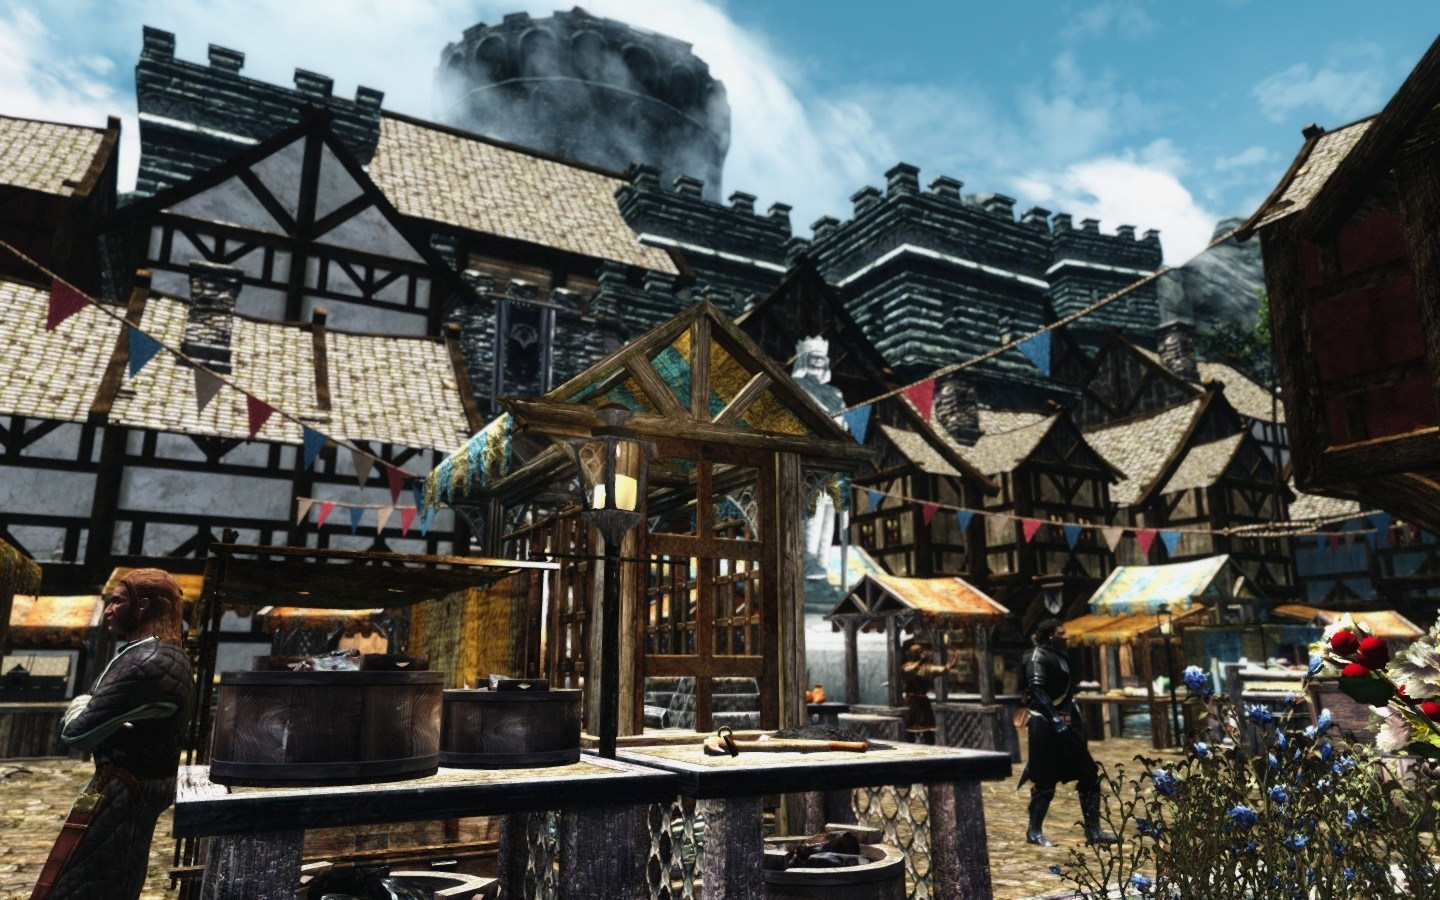
\includegraphics[width=\textwidth]{market.png}
\end{figure}
